Jenkins jest narzędziem automatyki open source napisanym w języku Java z wtyczkami zbudowanymi dla celów ciągłej integracji (ang. Continous Integration). Jenkins jest używany do budowania i testowania projektów oprogramowania w sposób ciągły, ułatwiając programistom integrowanie zmian w projekcie i ułatwiając użytkownikom uzyskanie nowej konstrukcji. Pozwala również na ciągłe dostarczanie oprogramowania poprzez integrację z dużą liczbą technologii testowych i wdrożeniowych.

Dzięki Jenkinsowi, organizacje mogą przyspieszyć proces tworzenia oprogramowania poprzez automatyzację. Jenkins integruje wszelkiego rodzaju procesy cyklu życia oprogramowania, w tym tworzenie, dokumentowanie, testowanie, pakowanie, etapowanie, wdrażanie, analizę statyczną i wiele innych.

W naszym przypadku Jenkins odpowiada za proces testowania oraz wdrożeniowy. Udane testy wysyłaja zapytanie o chęć wdrożenia najnowszej zmiany. Po pozytywnym rozpatrzeniu wysyłane jest odpowiednie zdarzenie do wcześniej przedstawionej platformy forge która zajmuje się wgraniem na serwer najnowszej wersji oprogramowania (rys. \ref{fig:jenkins}).

\begin{figure}[H]
    \centering
    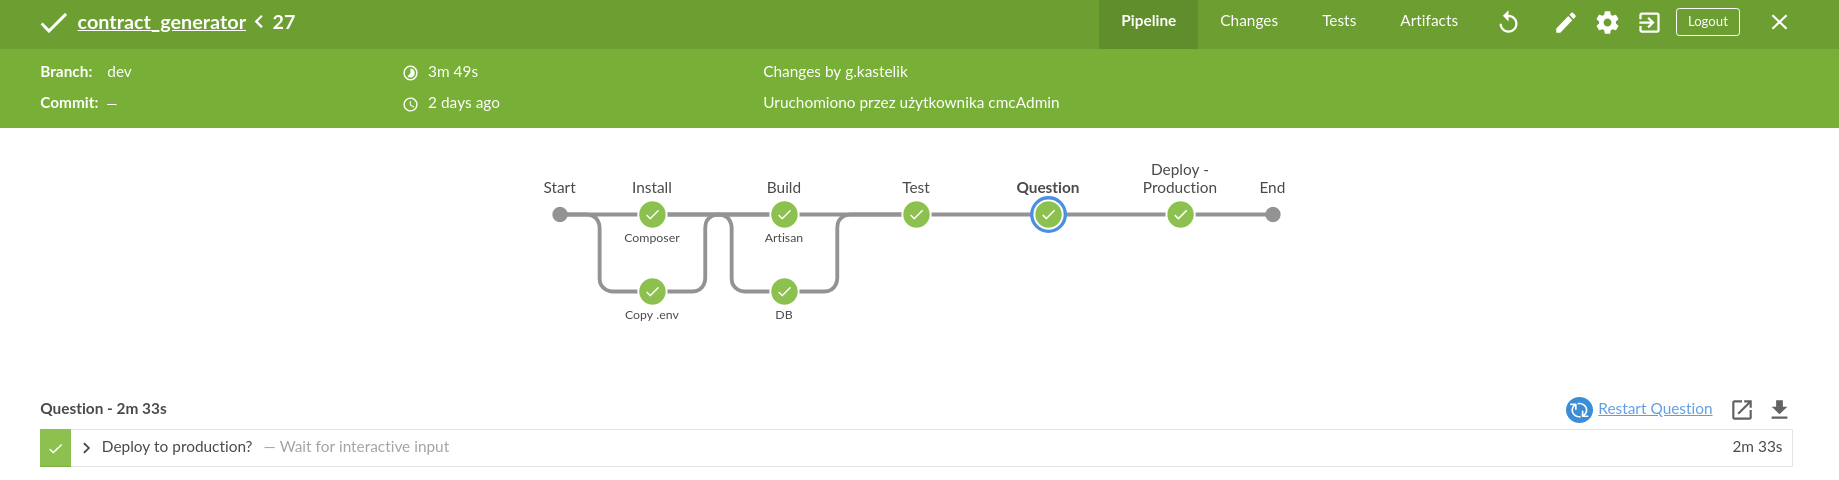
\includegraphics[width=6in]{images/jenkins.png}
    \caption{Proces testowania i wdrażania aplikacji \label{fig:jenkins}}
\end{figure}

\begin{figure}[H]
    \centering
    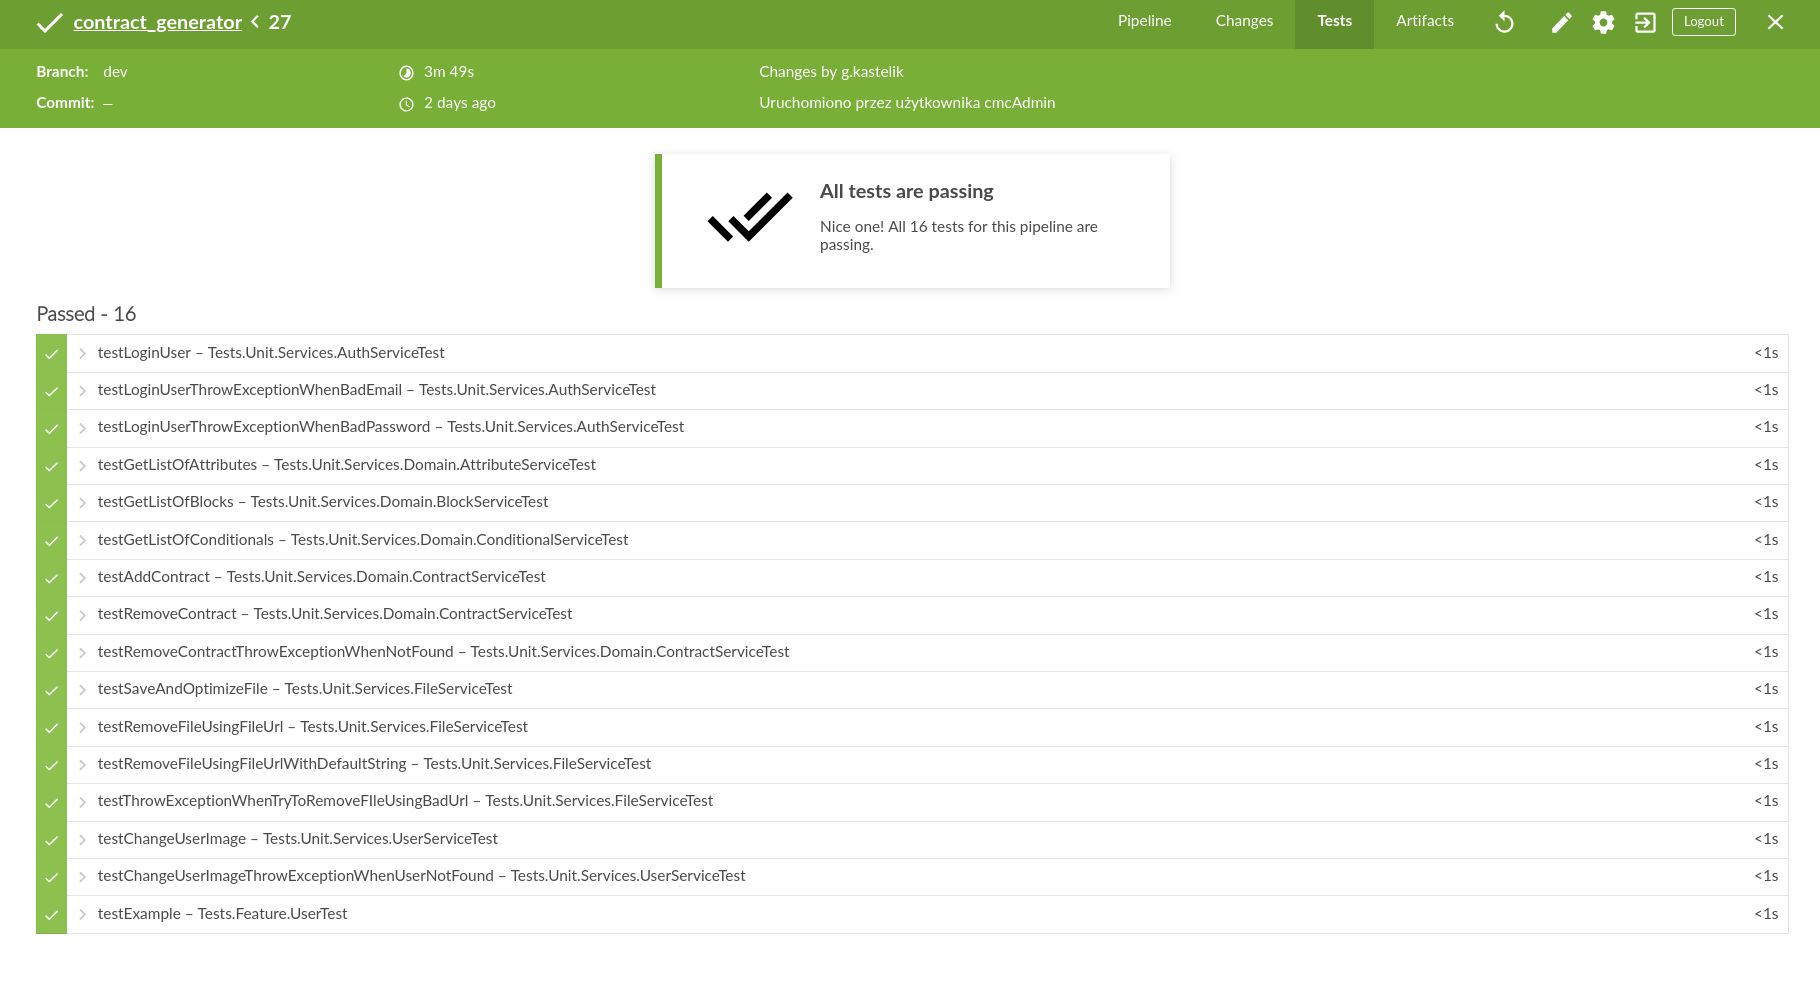
\includegraphics[width=6in]{images/jenkins-test.png}
    \caption{Raport na temat testów przeprowadzonych na aplikacji \label{fig:jenkins-test}}
\end{figure}

